\documentclass[]{report}

\usepackage[a4paper, left=1.5cm, right=1.5cm, top=2.5cm, bottom=1.5cm]{geometry} % imposta le dimensioni della pagina
\usepackage{multicol}
\usepackage{tocloft}
\usepackage[]{lipsum}
\usepackage[]{pgf-umlcd}
\usepackage{pgf-umlsd}
\usepackage{fontspec}


\usepackage{hyperref} % permette agli hypertext di essere cliccabili
\hypersetup{
    pdftitle={Progetto LSO},
    pdfauthor={Roberto Ingenito},
    colorlinks,
    linkcolor=black,
    citecolor=blue,
    filecolor=blue,
    urlcolor=blue
}

\usepackage{enumitem}
\setlist[itemize,enumerate]{
    topsep=0pt,
    itemsep=0pt,
    leftmargin=20pt
}
\usepackage[explicit]{titlesec}
\titleformat{\chapter}[display]{\Huge\bfseries}{\centering #1}{0pt}{}
% \renewcommand{\thesection}{\arabic{section}}
\titlespacing*{\subsection}{0pt}{30pt}{5pt}
\titlespacing*{\subsubsection}{0pt}{10pt}{2pt}

\usepackage{fancyhdr}
\pagestyle{fancy}
\fancypagestyle{plain}{%
  \renewcommand{\headrulewidth}{0pt}%
  \fancyhf{}%
}
\fancyfoot{}
\renewcommand{\chaptermark}[1]{\markboth{#1}{}}
\renewcommand{\sectionmark}[1]{\markright{#1}{}}
\fancyhead[L]{\leftmark}
\fancyhead[C]{}
\fancyhead[R]{\thepage}
\newcommand{\sskip}{\smallskip \\ }
\newcommand{\meskip}{\medskip \\ }
\newcommand{\bskip }{\bigskip \\ }

% \let\oldchapter\chapter
% \renewcommand{\chapter}[1]{
%     \newpage
%     \begingroup%
%     \let\clearpage\relax% Stop LaTeX from going to a new page
%     \vspace*{\fill}%
%     \oldchapter{#1}
%     \vspace*{\fill}%
%     \endgroup
%     \thispagestyle{empty}
%     \newpage
% }
% \let\oldsection\section
% \renewcommand{\section}[1]{
%     \newpage
%     \oldsection{#1}
% }

\linespread{1.2} % imposta lo spazio tra le righe
\fontdimen2\font=0.5em % imposta spazio tra le parole

\title{\textbf{Progetto LSO}\\Libreria}
\author{
    Ingenito Roberto - N86004077\\
    Ingenito Simone - N86004063\\
    Sequino Lorenzo - N86004367 
   }
\date{}


\begin{document}

\maketitle

\newpage

\clearpage\pagestyle{empty}
\begin{center}
	{\Huge\bfseries Indice\bigskip}
\end{center}

\setlength\columnsep{40pt}
% \setlength{\columnseprule}{1pt} % divider
\begin{multicols*}{2}
	\makeatletter
	\@starttoc{toc}
	\makeatother
\end{multicols*}
\clearpage\pagestyle{fancy}


\newpage
\chapter{Analisi dei requisiti}
\section{Obiettivo del progetto}
\section{Funzionalità principali}
\subsection{Registrazione e login utenti}
\subsection{Gestione del catalogo dei libri}
\subsection{Prestito di libri}
\subsection{Gestione del carrello e check-out}
\subsection{Notifiche agli utenti}

\chapter{Implementazione}
\section{Linguaggi di programmazione utilizzati}
C e SQL

\section{Struttura del codice}
Il progetto è organizzato in una struttura di cartelle che separa logicamente i vari componenti del progetto.\\
Questa organizzazione aiuta a mantenere il codice pulito, modulare e facile da gestire.\meskip
Di seguito, è riportata la struttura gerarchica delle cartelle:
\begin{verbatim}
    project_root
    +-- client
    |   +-- build
    |   +-- include
    |   +-- src
    +-- config
    +-- database
    |   +-- include
    |   +-- query
    |   +-- src
    +-- server
        +-- build
        +-- include
        +-- src
\end{verbatim}

\subsubsection*{\underline{client / server}}
Le cartelle \texttt{client} e \texttt{server} hanno la stessa struttura:
\begin{itemize}
	\item \texttt{\textbf{build}}: Contiene i file oggetto generati dalla compilazione del codice contenuto in \texttt{src}
	\item \texttt{\textbf{include}}: Contiene i file header
	\item \texttt{\textbf{src}}: Contiene il codice sorgente
\end{itemize}
La separazione tra \texttt{include} e \texttt{src} permette una chiara distinzione tra le interfacce e le implementazioni, migliorando la manutenibilità del codice. \\
La cartella build isola i file generati dalla compilazione, mantenendo pulito il repository.

\subsubsection*{\underline{config}}
Questa cartella possiede dei file di configurazione con implementazioni comuni sia per il \textit{client} che per il \textit{server}.\\
Ad esempio la configurazione del database, le richieste che client e server possono (rispettivamente) fare e ricevere, oppure la configurazione degli indirizzi.\meskip
Centralizzare le configurazioni in una cartella dedicata facilita la gestione delle impostazioni del sistema e permette di modificare facilmente i parametri di configurazione senza dover cercare all'interno del codice sorgente.

\subsubsection*{\underline{database}}
\begin{itemize}
	\item \texttt{\textbf{include}}: Contiene i file header per la gestione del database.
	\item \texttt{\textbf{query}}: Contiene i file SQL utilizzati per la gestione del database. (Creazione delle tabelle, trigger, funzioni, viste, \dots)
	\item \texttt{\textbf{src}}: Contiene il codice sorgente per l'interazione con il database.
\end{itemize}
La separazione dei file SQL e del codice sorgente relativo al database aiuta a mantenere organizzate le operazioni di gestione del database e facilita eventuali modifiche o aggiornamenti.






\section{Registrazione e login}
\subsection*{Client}
\subsection*{Server}

\section{Gestione dei libri e del catalogo}
\subsection*{Client}
\subsection*{Server}

\section{Prestito e restituzione libri}
\subsection*{Client}
\subsection*{Server}

\section{Carrello e check-out}
\subsection*{Client}
\subsection*{Server}

\section{Gestione delle notifiche}
\subsection*{Client}
\subsection*{Server}





\chapter{Database}
\section{Schema}
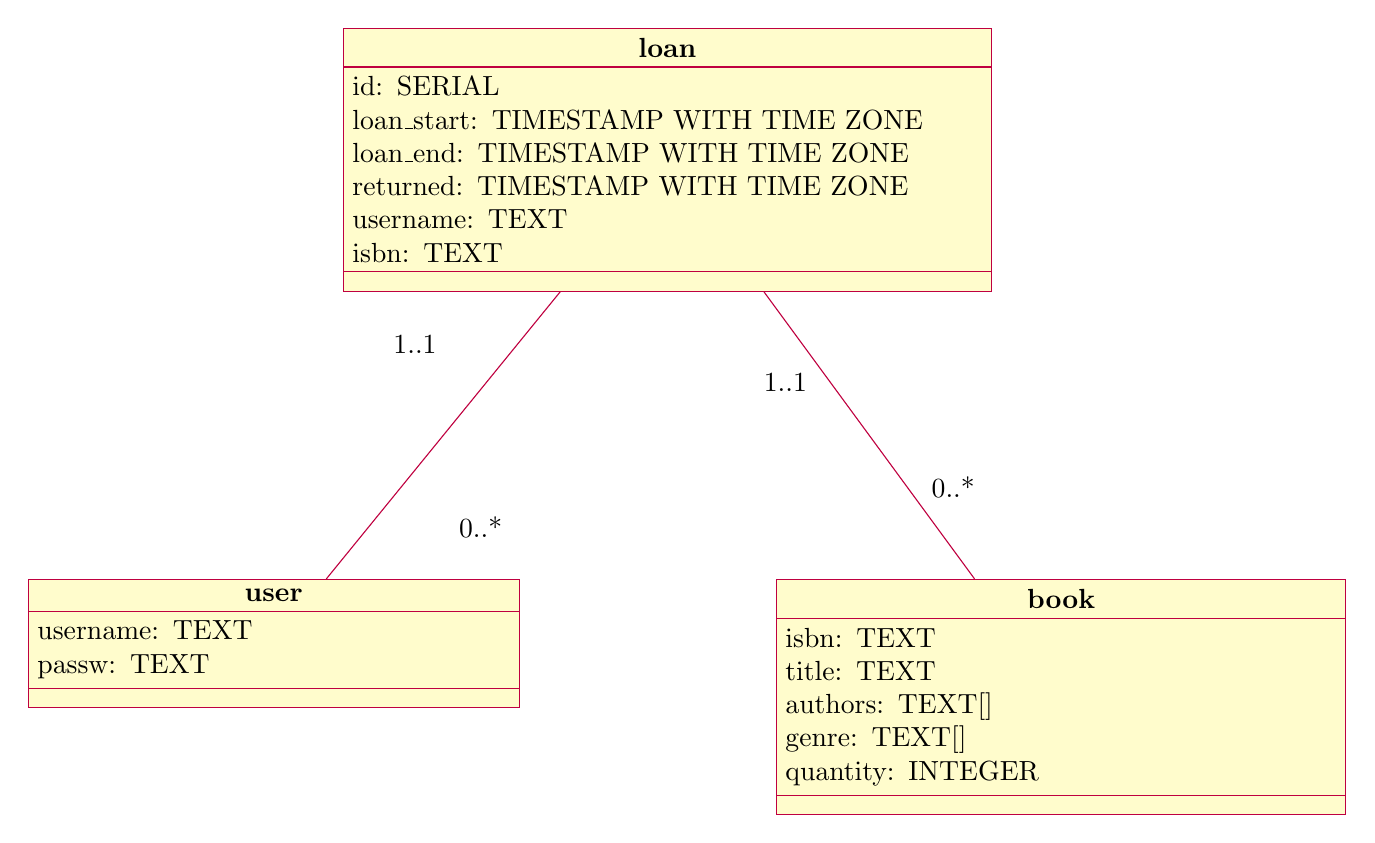
\begin{tikzpicture}
	% User table
	\begin{class}[text width=6cm]{user}{0,-7}
		\attribute{username: TEXT}
		\attribute{passw: TEXT}
	\end{class}

	% Book table
	\begin{class}[text width=7cm]{book}{10,-7}
		\attribute{isbn: TEXT}
		\attribute{title: TEXT}
		\attribute{authors: TEXT[]}
		\attribute{genre: TEXT[]}
		\attribute{quantity: INTEGER}
	\end{class}

	% Loan table
	\begin{class}[text width=8cm]{loan}{5,0}
		\attribute{id: SERIAL}
		\attribute{loan\_start: TIMESTAMP WITH TIME ZONE}
		\attribute{loan\_end: TIMESTAMP WITH TIME ZONE}
		\attribute{returned: TIMESTAMP WITH TIME ZONE}
		\attribute{username: TEXT}
		\attribute{isbn: TEXT}
	\end{class}

	% Relationships
	\association{user}{}{~\qquad0..*}{loan}{1..1\qquad~}{}
	\association{book}{}{0..*\qquad~}{loan}{~\qquad1..1}{}
\end{tikzpicture}

\section{Descrizione delle tabelle}
\section{Query principali utilizzate}


\end{document}




